Commenting system is providing a function for user to communicate and see what they are feeling in for our product xxxxx.\par~

There are three parts of the function shown below.
\textbf{Grading system}
Grading system is the part for the user to express their feeling and show their satisfaction with our product.\par~

There are five stars for the grade. The user could click the button of the stars from left to right. After they clicked the button, the star buttons(s) is/are coloured. The user could click the most left that is the most unsatisfying star, while the most right that is showing the most satisfying.

\textbf{Reply system}
Reply system is the part for the user to leave a message.\par~

User could leave any comment in comment box which is less than 1000 words. There are three buttons below the commenting box that user could click to choose whether showing to the public, private or only for the administrator. the public option is for the user to share their ideas. The private option is for the user to make a remark for there own. The administrator option is for the user to make any suggestions to the system for further development of our product.

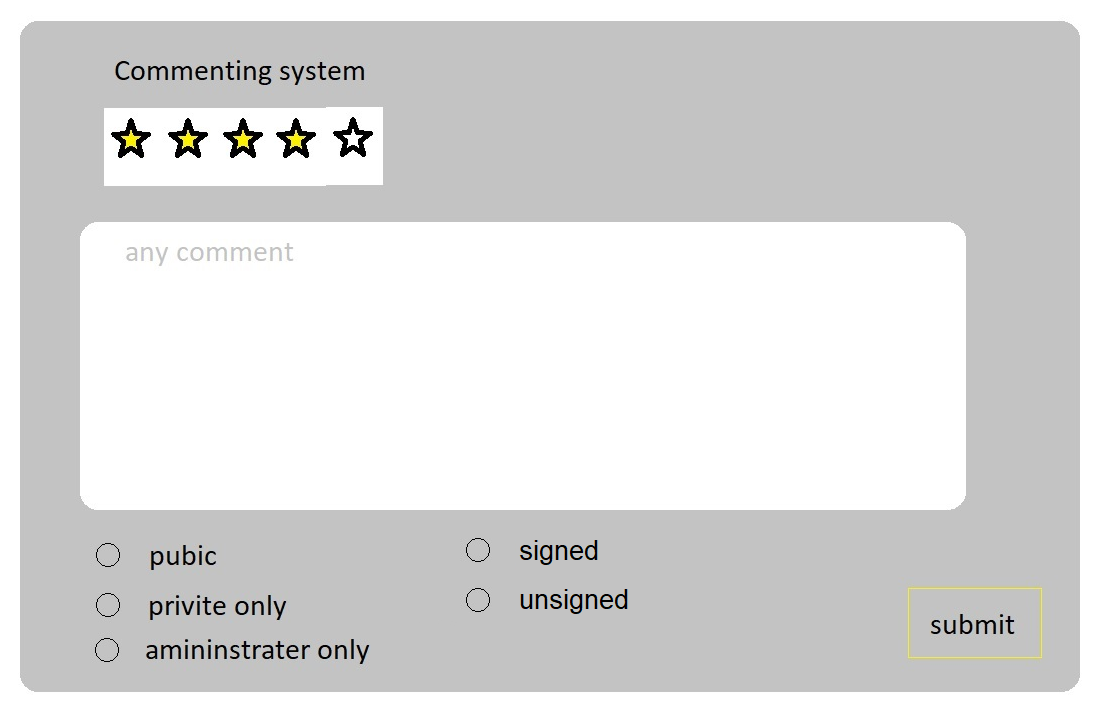
\includegraphics[scale=0.5]{Doc/Graphics/sdfg}

\textbf{Deleting system}
Deleting system is the part for the user to strike out useless message.\par~

The user could delete the comment by clicking the delete button which is on the right top corner.

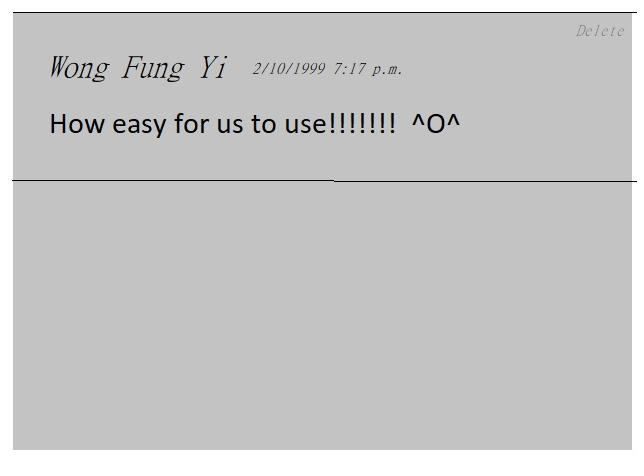
\includegraphics[scale=0.5]{Doc/Graphics/asdf}
